Alternative data visualization techniques can be found using the power of barycentric coordinates and GPU programming.

The usual way to visualize data for a triangle mesh is to associate data to vertices and then interpolating over the mesh triangles, that does not work in case of edges and triangles.

\section{Region around a vertex}
We can split the surface of triangle meshes into regions around vertex (Fig. \ref{fig:vertex-area}) and color them.

These regions can be determined using barycentric coordinates and GPU fragment program. Visualizing data given at the vertices or edges of the mesh in a piecewise constant simulates the classical triangle flat shading.
An example of this vertex data is the discrete Gaussian curvature.
\begin{figure}[h]
    \centering
    \minipage[b]{.4\linewidth}
    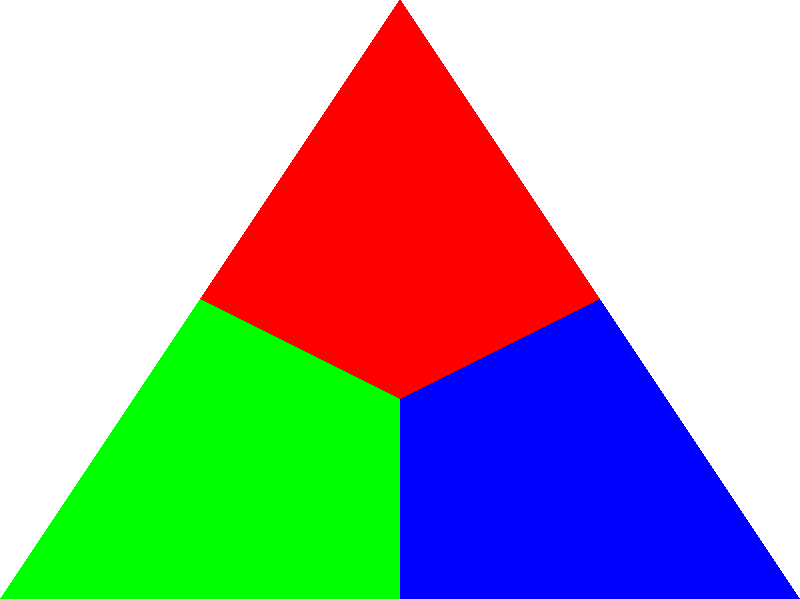
\includegraphics[scale=0.15]{images/max.png}
    \caption{Vertex based area}\label{fig:max-diagram}
    \endminipage\hfill
    \minipage[b]{.4\linewidth}
    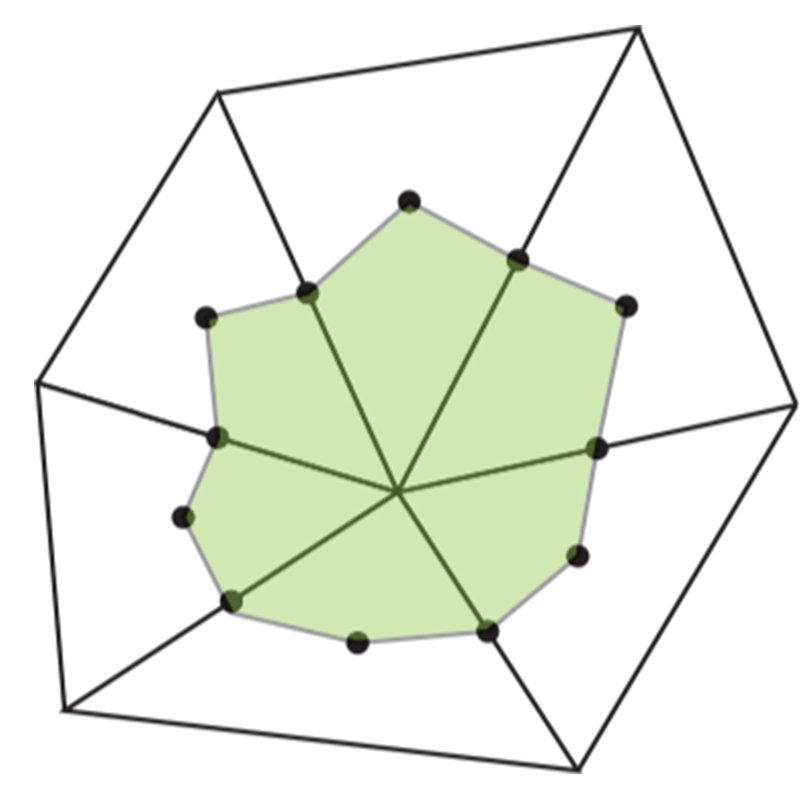
\includegraphics[scale=0.15]{images/vertex-area.png}
    \caption{Region around a vertex}\label{fig:vertex-area}
    \endminipage
\end{figure}


\subsection{Max diagram - Vertex based area} \label{section:max-diagram}
Passing barycentric coordinates to the fragment shader will clearly demonstrate that we can get results different from the classic color interpolation.

There are different approaches to color interpolation focusing on the distance from vertices. For each point in a triangle, we can easily determine its closest vertex, which we use as a cue for coloring.

A different approach from interpolating, can be found coloring vertex areas based on the minimum barycentric coordinate.
The color is given by the region farthest from a vertex (Fig. \ref{fig:max-diagram}).

\begin{lstlisting}[language=C++,
    directivestyle={\color{black}}
    emph={int,char,double,float,unsigned},
    emphstyle={\color{blue}}
   ]
if (Coords.x > Coords.y && Coords.x > Coords.z) {
    vec3 blue = vec3(0.0f, 0.0f, 1.0f);
    FragColor = vec4(blue, 1.0f);
} else if(Coords.y > Coords.x && Coords.y > Coords.z) {
    vec3 green = vec3(0.0f, 1.0f, 0.0f);
    FragColor = vec4(green, 1.0f);
} else {
    vec3 red = vec3(1.0f, 0.0f, 0.0f);
    FragColor = vec4(red, 1.0f);
}
\end{lstlisting}

\section{Color vertex area by lighting}
Suppose now that you want each vertex area to be in one constant color. This color can be taken from shading interpolation using the normal at the vertex and the vertex position. Then you can compute the color has it be done in \textit{Gouraud Shading}.

The idea is to compute the color per vertex but instead of linearly interpolated it in each triangle (as \textit{Gouraud shading} does) we color regions around a vertex with that constant color.

To implement that we need to pass the barycentric coordinates, the vertex color, the normal at the vertex and the lighting calculations to the \textit{fragment shader}.

We want to avoid an automatic interpolation of colors, in order to return the resulting color using the \textit{max diagram}, to do that we have used a \textit{Geometry shader} in order to access to all three vertex colors in fragment shader.
\\
\\
Vertex Shader for extend flat shading:
\begin{lstlisting}[language=C++,
    directivestyle={\color{black}}
    emph={int,char,double,float,unsigned},
    emphstyle={\color{blue}}
   ]
    #version 330 core
    layout (location = 0) in vec3 aPos;
    layout (location = 1) in vec3 aNormal;
    layout (location = 2) in vec3 aColor;

    struct Light {
        // ...
    };

    out vec4 vertex_color;

    uniform mat4 model;
    uniform mat4 view;
    uniform mat4 projection;

    void main() {
        vec3 world_position = vec3(model * vec4(aPos, 1.0));
        vec3 world_normal = mat3(transpose(inverse(model)))
                            * aNormal;

        // color obtained with lighting calculations
        vertex_color = get_result_color_lighting(...);

        gl_Position = projection * view
                      * model * vec4(aPos, 1.0);
    }
\end{lstlisting}

Geometry Shader for extend flat shading:
\begin{lstlisting}[language=C++,
    directivestyle={\color{black}}
    emph={int,char,double,float,unsigned},
    emphstyle={\color{blue}}
   ]
    #version 330 core
    layout (triangles) in;
    layout (triangle_strip, max_vertices = 3) out;

    in vec4 vertex_color[3];
    out vec3 coords;
    out vec4 wedge_color[3];

    void main() {
        wedge_color[0] = vertex_color[0];
        wedge_color[1] = vertex_color[1];
        wedge_color[2] = vertex_color[2];

        coords = vec3(1.0, 0.0, 0.0);
        gl_Position = gl_in[0].gl_Position;
        EmitVertex();

        coords = vec3(0.0, 1.0, 0.0);
        gl_Position = gl_in[1].gl_Position;
        EmitVertex();

        coords = vec3(0.0, 0.0, 1.0);
        gl_Position = gl_in[2].gl_Position;
        EmitVertex();

        EndPrimitive();
    }
\end{lstlisting}

Fragment Shader for extend flat shading:
\begin{lstlisting}[language=C++,
    directivestyle={\color{black}}
    emph={int,char,double,float,unsigned},
    emphstyle={\color{blue}}
   ]
    #version 330 core
    in vec3 coords;
    in vec4 wedge_color[3];
    out vec4 fragColor;

    void main() {
        // max diagram
        if (coords[0] > coords[1]) {
            if (coords[0] > coords[2]) {
                fragColor = wedge_color[0];
            }
            else {
                fragColor = wedge_color[2];
            }
        }
        else {
            if (coords[1] > coords[2]) {
                fragColor = wedge_color[1];
            }
            else {
                fragColor = wedge_color[2];
            }
        }
    }
\end{lstlisting}

\section{Color vertex area by Gaussian Curvature}
We want to compute the \textit{Gaussian curvature} per vertex. We want to sum up, for each vertex, angles at this vertex with adjacent triangles and then we subtract this value to $2\pi$.
After having obtain this value, called \textit{angle defect} (Fig. \ref{fig:gc-angle}), we map linearly this value to a color range.

Then we can pass this color to the \textit{vertex shader} to see the color vertex flat shading visualisation of Gaussian curvature.
$$G = 2\pi - \sum_j \theta_j$$
\begin{figure}[!h]
    \centering
    \begin{tikzpicture}
        \coordinate (J) at (3.1,2.9);
        \coordinate (circle) at (3.1,2.9);
        \node[anchor=south west,inner sep=0] at (0,0) {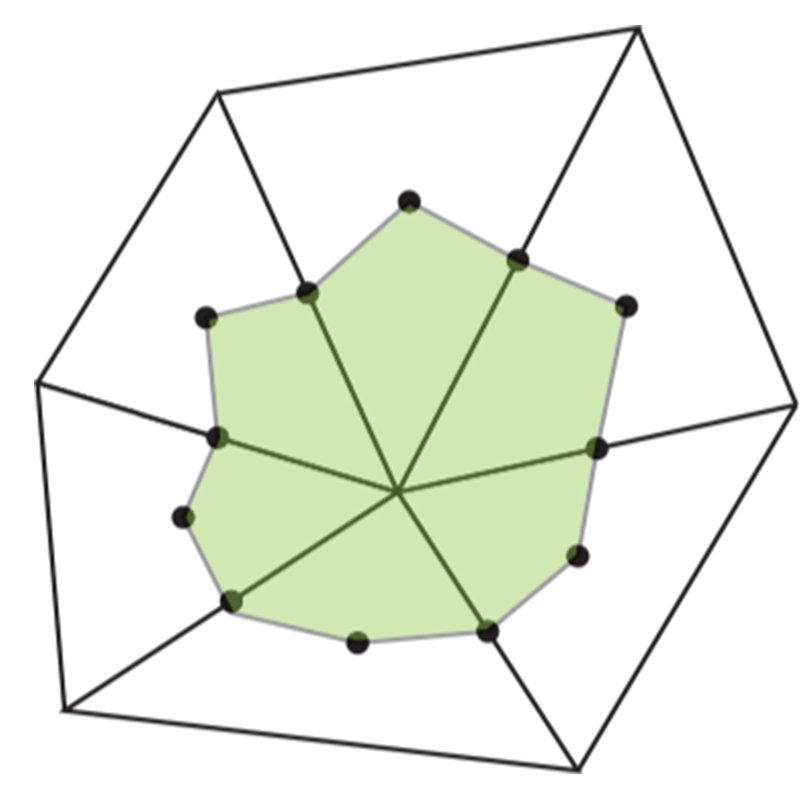
\includegraphics[scale=0.2]{images/vertex-area.png}};
        \draw (J) node [below left] {$j$};
        \filldraw (2.8, 2.2) circle (2pt);
        \begin{scope}[line width=0.4mm, line cap=round]
            \draw (3.2,1.7) arc (295:360:0.7cm) node[near start,right] {$\theta_j$};
        \end{scope}
    \end{tikzpicture}
    \caption{Angle defect}\label{fig:gc-angle}
\end{figure}

\textit{Gaussian curvature} should return a constant color around each vertex (Fig. \ref{fig:gc-icosahedron}).
\begin{figure}[h]
    \centering
    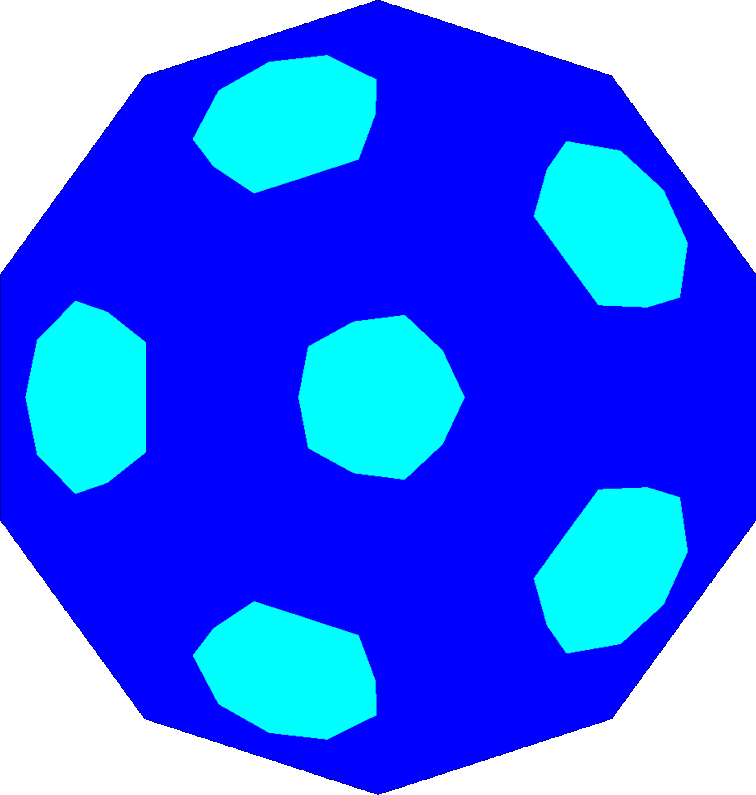
\includegraphics[scale=0.2]{images/gaussian-ball.png}
    \caption{Gaussian curvature on icosahedron}\label{fig:gc-icosahedron}
\end{figure}
\\
\\
Vertex Shader for gaussian curvature:
\begin{lstlisting}[language=C++,
    directivestyle={\color{black}}
    emph={int,char,double,float,unsigned},
    emphstyle={\color{blue}}
   ]
    #version 330 core
    layout (location = 0) in vec3 aPos;
    layout (location = 2) in vec3 gaussian_curvature;

    out vec4 vertex_color;

    uniform mat4 model;
    uniform mat4 view;
    uniform mat4 projection;

    uniform float min_gc;
    uniform float max_gc;
    uniform float mean_negative_gc;
    uniform float mean_positive_gc;


    vec3 interpolation(vec3 v0, vec3 v1, float t) {
        return (1 - t) * v0 + t * v1;
    }

    vec4 get_result_color_gc() {
       float val = gaussian_curvature[0];
       vec3 red = vec3(1.0, 0.0, 0.0);
       vec3 green = vec3(0.0, 1.0, 0.0);
       vec3 blue = vec3(0.0, 0.0, 1.0);

       //negative numbers until 0 -> map from red to green
       if (val < 0) {
            return vec4(interpolation(red, green,
                val/min_gc)/(mean_negative_gc/5), 1.0);
        } else {
            //map from green to blue, from 0 to positive
            return vec4(interpolation(green, blue,
                val/max_gc)/(mean_positive_gc/5), 1.0);
        }
    }

    void main() {
        vec3 pos = vec3(model * vec4(aPos, 1.0));

        vertex_color = get_result_color_gc();

        gl_Position = projection * view * model *
                      vec4(aPos, 1.0);
    }
\end{lstlisting}

\section{Evaluation and Comparison}
We want now to compare the classic linear interpolation visualisation (Fig. \ref{fig:interpolation-horse}) with two possible way to extend the flat shading. In Fig. \ref{fig:lighting-horse} and Fig. \ref{fig:gaussian-horse} we have color each vertex area following the method \textit{max diagram} described in the above subsection \ref{section:max-diagram}, this extension of the flat shading returns a more 3-dimensional model.
In fact, as we can see in Fig. \ref{fig:lighting-horse} and Fig. \ref{fig:gaussian-horse}, the horse get more realistic thanks to the lighting calculation for Fig. \ref{fig:lighting-horse} and to the \textit{Gaussian curvature} for Fig. \ref{fig:gaussian-horse}, in particular this last result in a more detailed model.
\begin{figure}[!htb]
  \minipage{0.32\textwidth}
    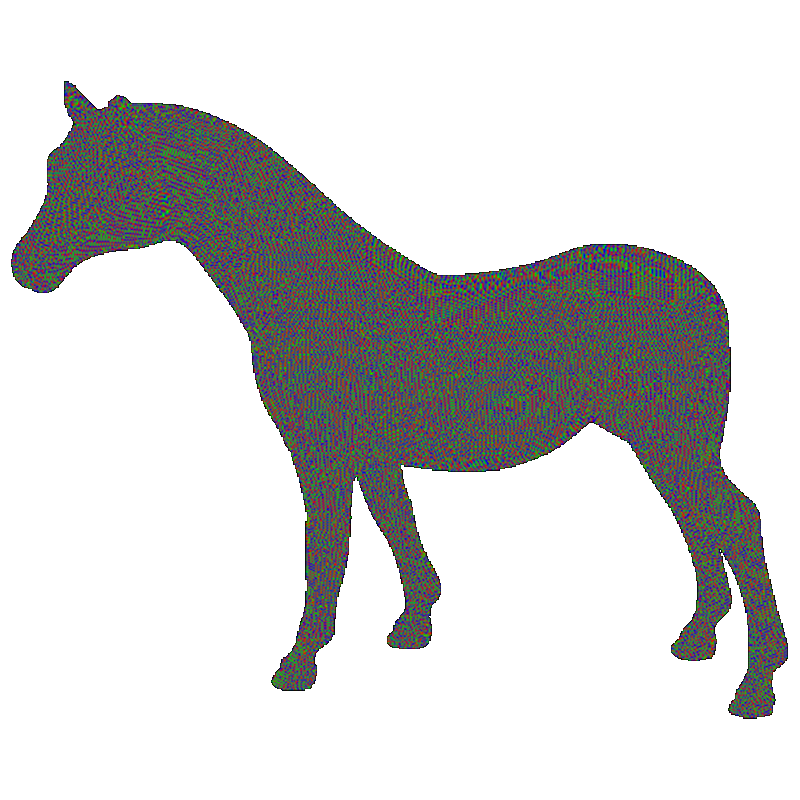
\includegraphics[width=\linewidth]{images/linear-horse.png}
    \caption{Interpolation}\label{fig:interpolation-horse}
  \endminipage\hfill
  \minipage{0.32\textwidth}
%     \includegraphics[width=\linewidth]{flat.png}
    \caption{Lighting calculation}\label{fig:lighting-horse}
  \endminipage\hfill
  \minipage{0.32\textwidth}%
    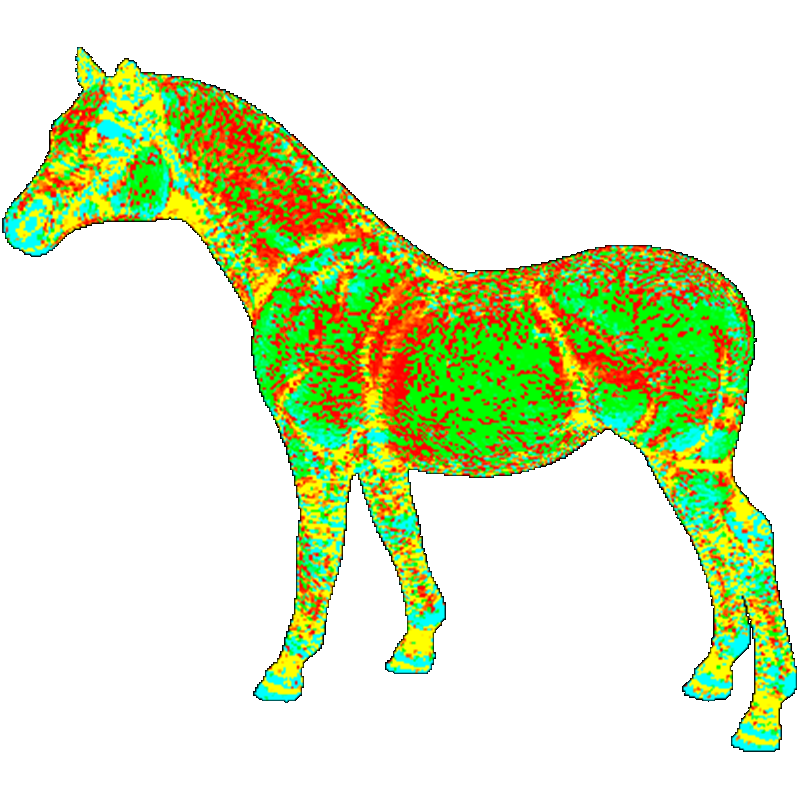
\includegraphics[width=\linewidth]{images/gaussian-horse.png}
    \caption{Gaussian Curvature}\label{fig:gaussian-horse}
  \endminipage
  \end{figure}
  Visualization of the principal curvatures as colors (Fig. \ref{fig:gaussian-horse}), marking then every change of signs highlighting the 3-dimensionality of the model.
